\chapter{Podatkovne zbirke Svetovne Banke}

Pri diplomski nalogi smo se osredotočili na dva programska vmesnika za dostop 
podatkov Svetovne banke, to sta ``ClimateAPI'' s katerim dostopamo do 
podatkovne zbirke meteoroloških meritev in ``IndicatorAPI'' s katerim dostopamo do 
zbirke podatkov raznih indikatorjev stopenj razvoja držav.
Za uporabo podatkovne zbirke Svetovne banke smo se odločili, ker združuje in na
enovit način predstavi podatke iz več različnih virov. Podatkovni viri za 
indikatorje stopnje razvoja držav so:
\begin{itemize}  
  \item Svetovni indikatorji razvoja~\cite{world_dev_ind} % World Development Indicators, 
  \item Globalni finančni razvoj~\cite{glob_fin_dev}
  \item Afriški indikatorji razvoja~\cite{africa_dev_ind}
  \item Poslovanje~\cite{doing_buseness},
  \item Podjetniške raziskave~\cite{ent_surveys}, 
  \item Razvojni cilji~\cite{mil_dev_goals}, 
  \item Statistike izobraževanja~\cite{edu_stat}, 
  \item Statistike spolov~\cite{gen_stat},
  \item Statistike zdravja in prehranjevanja~\cite{health_pop_stat},
  \item Rezultati meritev IDA~\cite{ida_res_mes_sys}.
\end{itemize}  

Podatkovni vir zbirke podnebnih meritev pa je osnovan na podatkih oddelka
za podnebne raziskave (ang.\ Climatic Research Unit)~\cite{climate_data}.

Svetovna banka omogoča dostop do podatkov preko programskega vmesnika REST, ki
ponuja veliko možnosti za iskanje in presejanje rezultatov. Pri vsaki 
poizvedbi REST lahko določimo želeno obliko odgovora. Za poizvedbe o 
informacijah indikatorjev sta na voljo obliki XML in JSON. Programski vmesnik 
meteoroloških meritev pa ponuja samo obliko JSON. Za konsistentnost in lažjo
berljivost smo na obeh programskih vmesnikih uporabili obliko JSON. To na
programskem vmesniku indikatorjev dosežemo tako da nastavimo parameter GET
\verb|format| na vrednost \verb|json|. 


\section{Podatki indikatorjev razvoja držav}
\label{sec:podatki_ind_razvoja}



Programski vmesnik indikatorjev razvoja držav Svetovne banke omogoča dostop
do podatkov preko 16.000 raznih indikatorjev. Podatki indikatorjev so merjeni v
mesečnem, četrtletnem ali letnem intervalu. Začetek meritev podatkov
posameznega indikatorja je odvisna od vira podatkov. Najstarejši podatki segajo
do leta 1960. Poleg podatkov indikatorjev nam ta programski vmesnik omogoča 
tudi dostop do večine metapodatkov, s katerimi lahko presejamo in natančneje
določimo našo poizvedbo. Seznami metapodatkov so:
\begin{itemize}
\item viri podatkov in njihovi opisi (ang.\ Catalog Source Queries
	\fnurl{http://api.worldbank.org/sources?format=json}),
\item seznam držav, skupin držav in regij z identifikatorji (ang.\ Country Queries
	\fnurl{http://api.worldbank.org/countries?format=json}),
\item razdelitev višin dohodkov z identifikatorji (ang.\ Income Level Queries
	\fnurl{http://api.worldbank.org/incomeLevels?format=json}),
\item seznam indikatorjev (ang.\ Indicator Queries
  \fnurl{http://api.worldbank.org/indicators?format=json}),
\item seznam tipov posojil (ang.\ Lending Type Queries
	\fnurl{http://api.worldbank.org/lendingTypes?format=json}),
\item seznam tem (ang.\ Topics \fnurl{http://api.worldbank.org/topics}).
\end{itemize}

Za pridobitev podatkov indikatorjev potrebujemo metapodatke o indikatorjih in
državah. Primere teh metapodatkov si bomo podrobneje pogledali v nadaljevanju.

Ker je mogoče z eno poizvedbo dostopati do velike količine podatkov, ima
programski vmesnik za dostop do podatkov indikatorjev implementirano
ostranjevanje, s katerim je omejeno število podatkov, ki jih lahko dobimo z eno
poizvedbo. Tako so podatki razdeljeni na skupine ki jih imenujemo strani.

Vsi odgovori na veljavne poizvedbe po podatkih in metapodatkih, ki so na voljo
s programskim vmesnikom indikatorjev razvoja, imajo enako osnovno obliko. 
Poizvedbe vračajo seznam z dvema elementoma, kjer ima prvi element 
informacije o količini podatkov in trenutnem izboru podatkov, drugi element 
pa vsebuje seznam izbranih podatkov (Primer \ref{basic_response}). Privzeta
vrednost števila elementov na stran je $50$, kar lahko spremenimo tako, da
poizvedbi nastavimo parameter GET \verb|per_page| na poljubno vrednost. Če
želimo pridobiti podatke z več strani, moramo za vsako stran poslati novo
poizvedbo, v kateri podamo želeno stran s parametrom GET \verb|page|, . 
Veljavne poizvedbe, s sitom ki ne vrača nobenih podatkov, imajo vrednost 
drugega elementa osnovnega seznama \verb|null|.
Za neveljavne poizvedbe pa programski vmesnik vrača seznam z enim elementom,
ki vsebuje podatke o napaki poizvedbe (Primer \ref{error_response}).


\begin{snippet}
\begin{center}
\begin{lstlisting}
[
    {
        'page': 1,
        'pages': 137,
        'per_page': '50',
        'total': 6831
    },
    [
        <podatki>,
        ...
    ]
]
\end{lstlisting}
\end{center}
\caption{Osnovna oblika odgovora programskega vmesnika Svetovne banke za
veljavno poizvedbo indikatorjev.} 
\label{basic_response}
\end{snippet} 


\begin{snippet}
\begin{center}
\begin{lstlisting}
[
    {
        'message': [
            {
                'id': '120',
                'key': 'Parameter \'country\' has an invalid value',
                'value': 'The provided parameter value is not valid'
            }
        ]
    }
]
\end{lstlisting}
\end{center}
\caption{Osnovna oblika odgovora programskega vmesnika Svetovne banke, za
neveljavne poizvedbe.}
\label{error_response}
\end{snippet} 


\subsection{Opis seznama indikatorjev}

Programski vmesnik Svetovne banke za indikatorje razvoja nam ponuja seznam 
vseh indikatorjev z imeni, opisi, kodami in drugimi metapodatki 
(Primer \ref{indicator_response}). Programski vmesnik nam omogoča tudi dostop
do podatkov posameznega indikatorja določenega s kodo in presejanje seznama 
indikatorjev glede na vir podatkov \ref{indicator_queries}. V našem programu
smo uporabili le poizvedbo za celoten seznam indikatorjev, da smo omogočili 
iskanje in presejanje po vseh poljih indikatorjev.

\begin{snippet}
\begin{center}
\begin{lstlisting}
http://api.worldbank.org/indicators?format=json
http://api.worldbank.org/indicators?format=json&source=5
http://api.worldbank.org/indicators/A10i?format=json
\end{lstlisting}
\end{center}
\caption{Primeri poizvedb po seznamu indikatorjev.
1) seznam vseh indikatorjev, 2) seznam indikatorjev glede na vir podatkov,
3) podatki indikatorja ``A10i''}
\label{indicator_queries}
\end{snippet} 


\begin{snippet}
\begin{center}
\begin{lstlisting}
{
    'id': '1.0.HCount.2.5usd',
    'name': 'Poverty Headcount (\$2.50 a day)',
    'source': {
        'id': '37',
        'value': 'LAC Equity Lab'
    },
    'sourceNote': 'The poverty headcount index measures the 
                   proportion of the population with daily per 
                   capita income (in  2005 PPP) below the poverty
                   line.',
    'sourceOrganization': 'LAC Equity Lab tabulations of SEDLAC 
                           (CEDLAS and the World Bank).',
    'topics': [
        {
            'id': '11',
            'value': 'Poverty '
        }
    ]
}
\end{lstlisting}
\end{center}
\caption{Podatki indikatorja 
% TODO
% Ali moram ime indikatorja oznaciti (naprimer velika zacetnica)
% > Podatki indikatorja Stopnja rev...
stopnja revščine pri dohodku 2,5 dolarja na dan.}
\label{indicator_response}
\end{snippet} 

\subsection{Opis seznama držav}

Seznam držav na programskem vmesniku Svetovne banke vsebuje podatke o imenih, 
opisih, ISO-3166-1 alpha kodah, regijah in druge metapodatke 
(Primer \ref{country_response}). Programski
vmesnik nam omogoča tudi presejanje seznama držav po kodi države, regiji,
višini dohodka in tipu posojil (Premer \ref{country_queries})

% \begin{description}
% \item [id] koda države, regije ali skupine držav,
% \item [region] regija,
% \item [incomeLevel] višina dohodka,
% \item [lendingType] tipov posojil. % TODO preveri prevod!
% \end{description}

\begin{snippet}
\begin{center}
\begin{lstlisting}
http://api.worldbank.org/countries?format=json
http://api.worldbank.org/countries/svn?format=json
http://api.worldbank.org/countries?format=json&incomeLevel=HIC&region=ECS
\end{lstlisting}
\end{center}
\caption{Primeri poizvedb po seznamu držav.
1) seznam vseh držav, 2) podatki ene države,
3) seznam držav v Evropi in Osrednji Aziji z visoko višino dohodka.}
\label{country_queries}
\end{snippet} 

Ta seznam ne vsebuje zgolj samo držav, ampak tudi regije in skupine držav, 
združenih glede na različne kriterije (višine dohodka, velikost, stopnja
razvoja). Poleg tega zgornji seznam vsebuje tudi nekatere izjeme kot je trenutno
Kosovo. V nadaljevanju bomo za vse naštete tipe lokacijskih podatkov
uporabljali besedo ``države''. 

\begin{snippet}
\begin{center}
\begin{lstlisting}
{
    'id': 'ABW',
    'iso2Code': 'AW',
    'name': 'Aruba',
    'region': {
        'id': 'LCN',
        'value': 'Latin America & Caribbean '
    },
    'adminregion': {
        'id': '',
        'value': ''
    },
    'incomeLevel': {
        'id': 'HIC',
        'value': 'High income'
    },
    'lendingType': {
        'id': 'LNX',
        'value': 'Not classified'
    },
    'capitalCity': 'Oranjestad',
    'longitude': '-70.0167',
    'latitude': '12.5167'
},
\end{lstlisting}
\end{center}
\caption[some]{Izsek podatkov veljavne poizvedbe držav.}
\label{country_response}
\end{snippet} 


\subsection{Dostop do podatkov indikatorjev}

Za dostop do podatkov posameznega indikatorja potrebujemo kodo
indikatorja s seznama vseh indikatorjev in kodo ene ali več držav. Namesto
kode ene ali več držav, lahko uporabimo tudi ključno besedo ``all'', ki
označuje vse kode držav. Pri večjih količinah podatkov lahko z dodatnimi
parametri določimo število podatkov na stran, in želeno stran podatkov.
Primer \ref{indicator_dataset_request} prikazuje osnovno obliko poizvedbe,
kjer so:
\begin{description}
\item [country] s podpičjem ločen seznam kod izbranih držav, ki jih 
	  preberemo iz polja ``id'' ali ``iso2Code'', ki sta prikazana v Primeru 
    \ref{country_response}, ali pa ključna beseda ``all'',
\item [indicator\_id] polje ``id'' indikatorja ki je prikazano v Primeru 
    \ref{indicator_response}.
\item [parametri] Dodatni parametri GET 
\end{description}
Za poizvedbe do podatkov indikatorjev so poleg osnovnih parametrov GET 
\verb|per_page|, \verb|page| in \verb|format|, opisanih v poglavju 
\ref{sec:podatki_ind_razvoja}, na voljo tudi dodatni parametri za presejanje
rezultatov poizvedbe:
\begin{description}  
\item [MRV] Številska vrednost, ki določi maksimalno število zadnjih meritev,
    ki jih programski vmesnik vrne. Ko uporabljamo polje \verb|mrv| bo 
    programski vmesnik izpustil ničelne vrednosti za obdobja v katerih ni
    meritev.
\item [gapfill] Zastavica \verb|'y'| ali \verb|'n'| za manjkajoče vrednosti meritev.
    Vrednost \verb|'y'| kombinaciji s poljem \verb|mrv| poskrbi da programski 
    vmesnik ne izpusti nobenega časovnega intervala.
\item [date] Polje oblike \verb|'leto'| ali \verb|'leto:leto'| ki omeji rezultate poizvedbe
    na določeno leto ali interval med določenimi leti. 
\end{description}


\begin{snippet}
\begin{center}
\begin{lstlisting}
http://api.worldbank.org/en/countries/<country>/indicators/<indicator_id>?<parametri>
\end{lstlisting}
\end{center}
\caption{Osnovna oblika poizvedbe za podatke enega indikatorja.}
\label{indicator_dataset_request}
\end{snippet} 

% http://api.worldbank.org/countries/svn/indicators/SL.TLF.ACTI.FE.ZS?format=json
% http://api.worldbank.org/countries/svn;usa/indicators/SL.TLF.ACTI.FE.ZS?format=json
% http://api.worldbank.org/countries/all/indicators/SL.TLF.ACTI.FE.ZS?format=json

Privzeta vrednost za količino podatkov na stran \verb|per_page| je 50. 
Zgornja meja pa ni strogo določena, vendar je odvisna od velikosti odgovora. 
Ugotovili smo, da se zanesljivost programskega vmesnika manjša z večjo 
količino podatkov na stran. V našem programu smo se omejili na 1000 podatkov
na stran, kar se je izkazalo za uporabno razmerje med hitrostjo in 
zanesljivostjo programskega vmesnika. Privzeto bo programski vmesnik vrnil 
podatke za vse časovne vrednosti. V odgovoru API-ja dobimo seznam objektov 
(Primer \ref{dataset_response}) z datumom, indikatorjem, državo in vrednostjo.

\begin{snippet}
\begin{center}
\begin{lstlisting}
{
    'indicator': {
        'id': 'SP.POP.TOTL',
        'value': 'Population, total'
    },
    'country': {
        'id': 'IL',
        'value': 'Israel'
    },
    'value': '6289000',
    'decimal': '0',
    'date': '2000'
}
\end{lstlisting}
\end{center}
\caption{Podatki za indikator SP.POP.TOTL (populacija države) za Izrael leta
2000.}
\label{dataset_response}
\end{snippet} 

Slabosti programskega vmesnika indikatorjev Svetovne banke za uporabo v namene
podatkovnega rudarjenja so v tem, da vmesnik ni namenjen prenosu večje 
količine podatkov z eno samo poizvedbo. Zaradi ostranjevanja moramo za en sam 
indikator narediti več poizvedb, da prenesemo podatke z vseh strani. Prav 
tako podatkovni vmesnik ne podpira poizvedb po več indikatorjih hkrati, kar
potrebujemo za iskanje zakonitosti med posameznimi indikatorji.

\section{Podatki podnebnih meritev}

Programski vmesnik Svetovne banke za podnebne podatke omogoča dostop do 
podatkov napovednih modelov in zgodovinskih meritev meteoroloških postaj. V tej 
diplomski nalogi smo se odločili uporabiti samo podatke zgodovinskih meritev, 
saj si s temi podatki lahko uporabnik programa Orange sam sestavi svoje 
napovedne modele.

Za razliko od uporabe programskega vmesnika indikatorjev, lahko pri tem
programskem vmesniku uporabljamo veljavne ISO 3166-1 alpha-2 ali ISO 3166-1 
alpha-3 kode držav, ali pa številski identifikator vodotočnega 
območja.

Ta programski vmesnik nam omogoča dostop do podatkov o povprečnih 
temperaturah in padavinah v časovnih obdobjih enega leta, desetletja ali pa 
nam omogoča dostop do mesečnih povprečij skozi vsa leta meritev.


\subsection{Dostop do podatkov podnebnih meritev}

Za dostop do podnebnih podatkov preko programskega vmesnika Svetovne banke
potrebujemo ISO-3166-1 alpha3 kodo države ali številski identifikator
vodotočnega območja (Slika \ref{climate_data_api_basins}). Programski vmesnik
nam omogoča dostop do meritev povprečnih količin padavin in temperatur za 
letno ali desetletno obdobje. Poleg letnega in desetletnega obdobja pa nam 
programski vmesnik ponuja tudi povprečno količino padavin in temperatur za 
posamezne mesece skozi vsa leta meritev. Obliko poizvedbe prikazuje primer 
\ref{climate_dataset_request}, kjer je:
\begin{description}
\item [loc\_type] vrsta identifikatorja območja (``basin'' za vodotočno območje, 
  ``country'' za države),
\item [data\_type] vrsta meritev (``pr'' za padavine, ``tas'' za temperature),
\item [interval] vrsta meritvenega obdobja (``month'' za mesečno, ``year'' za letno in
  ``decade'' za desetletno),
\item [location] koda države ali številski identifikator vodotočnega območja.
\end{description}
Za razliko od programskega vmesnika indikatorjev, nam programski vmesnik
podnebnih meritev z eno poizvedbo omogoča dostop do podatkov le za eno državo.
To pomeni, da je količina podatkov dovolj omejena, da nam programski vmesnik
vedno vrne vse podatke brez ostranjevanja, kot prikazuje primer 
\ref{climate_dataset_response},


\begin{figure}
\begin{center}
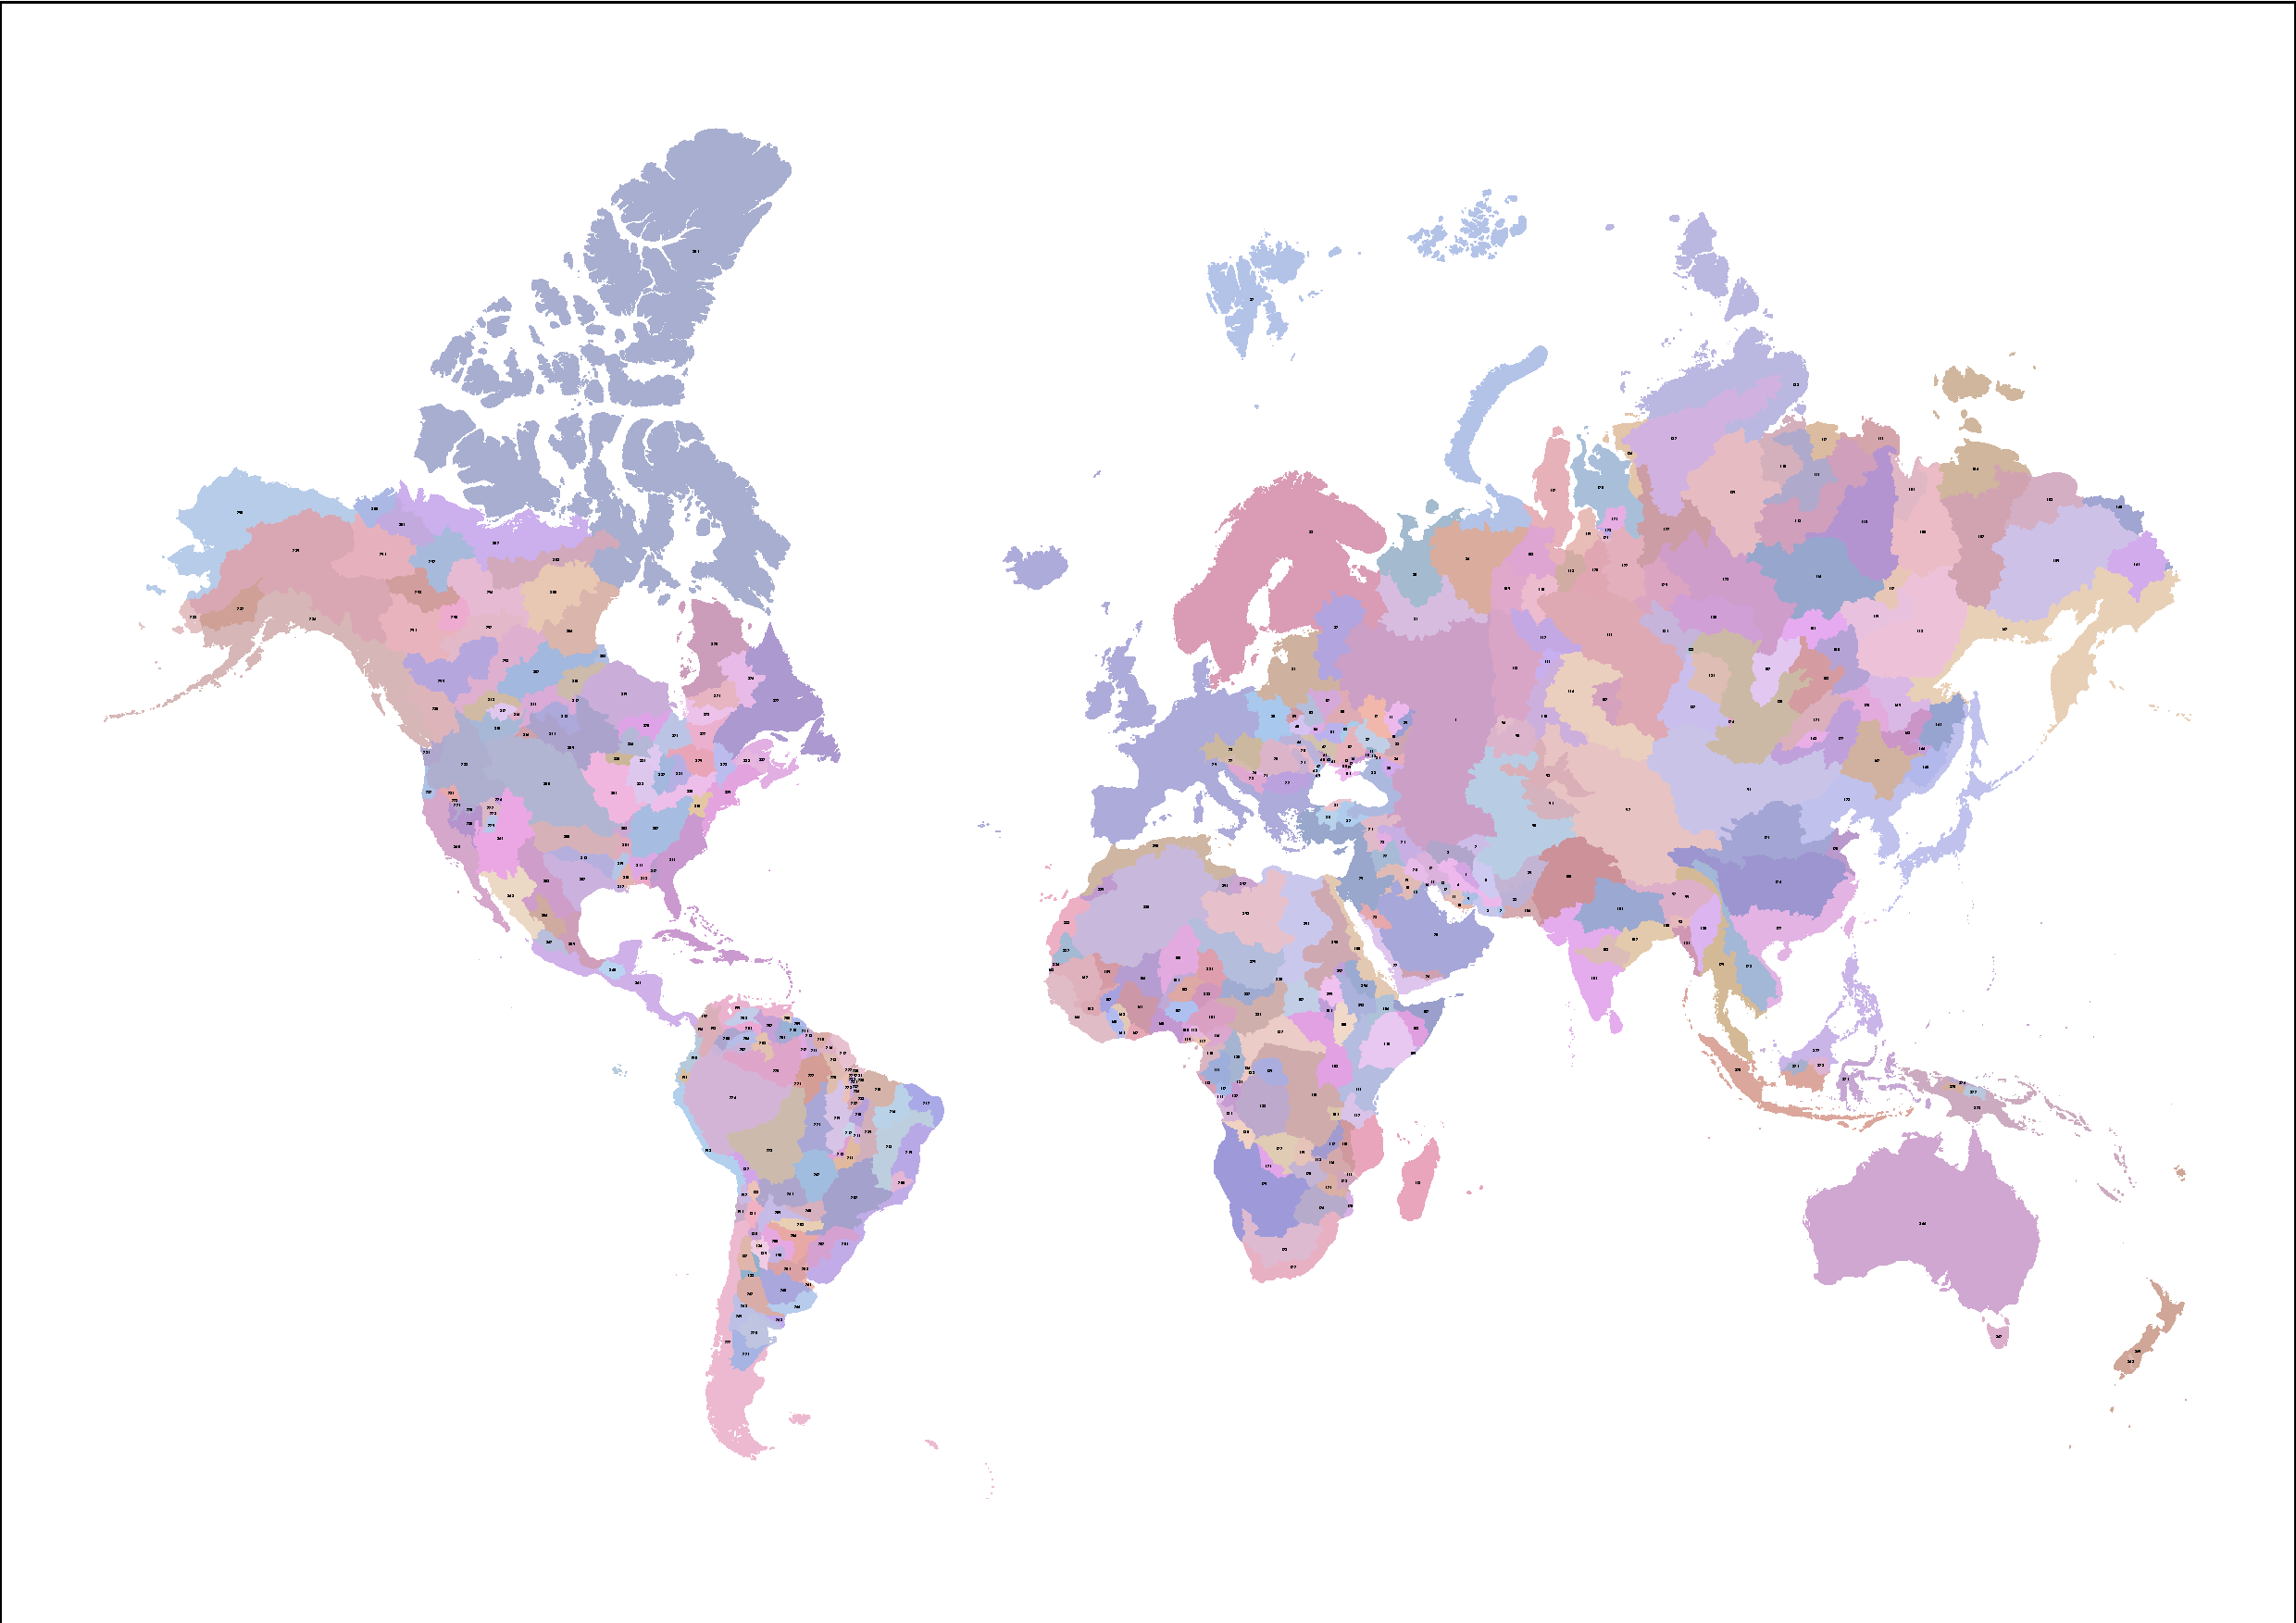
\includegraphics[width=12cm]{pic/climate_data_api_basins.pdf}
\end{center}
\caption{Prikaz vodotočnih območij sveta.}
\label{climate_data_api_basins}
\end{figure} 


\begin{snippet}
\begin{center}
\begin{lstlisting}
http://climatedataapi.worldbank.org/climateweb/rest/v1/<loc_type>/cru/<data_type>/<interval>/<location>
\end{lstlisting}
\end{center}
\caption{Osnovna oblika poizvedbe za podnebne podatke.}
\label{climate_dataset_request}
\end{snippet} 


\begin{snippet}
\begin{center}
\begin{lstlisting}
[
    {
        'month': 0,
        'data': 68.93643
    },
    {
        'month': 1,
        'data': 64.23069
    },
    {
        'month': 2,
        'data': 81.098724
    },
    ...
]
\end{lstlisting}
\end{center}
\caption{Primer odgovora za poizvedbo količine padavin v posameznih mesecih v 
  Sloveniji.}
\label{climate_dataset_response}
\end{snippet} 






\section{Težave pri uporabi programskih vmesnikov Svetovne banke}
\label{api_gotchas}


Programski vmesniki Svetovne banke zajemajo podatke iz različnih virov, zato je
težko zagotoviti pravilnost in konsistentnost podatkov. Poleg tega pa se 
programski vmesnik in spletna stran z dokumentacijo občasno spremenita, kar
povzroča še dodatne težave pri uporabi. Nekatere težave, ki smo jih opazili
so:
\begin{itemize}  
\item nekaterim delom dokumentacije se je med izdelavo te diplomske naloge
  spremenil spletni naslov, tako da do tistih delov sedaj nimamo več dostopa,
\item polje za datum v odgovoru je opisano, vendar ni dokumentirano, kakšne so
    vse možne vrednosti (nekaj primerov nedokumentiranih vrednosti:
    ``last known value'' ``2001 - 2015'' ``2040''),
\item delovanje sita z različnimi kombinacijami polj \verb|mrv|, \verb|gapfill|
  in \verb|date| ni ustrezno opisano,
\item v odgovoru poizvedbe po podatkih indikatorjev ponekod manjkajo vrednosti
  kot so koda države, ime države ali ime indikatorja.
\item zgornja meja števila izbranih lokacij na 250 ni navedena in napaka 
  ki jo programski vmesnik vrne ni dokumentirana,
\item nemogoče je ugotoviti pogostost vzorčenja indikatorja (frequency), .
\end{itemize}  







